\documentclass[10pt]{article}
\usepackage[margin=0.4in]{geometry}
\usepackage{amsmath}
\usepackage{enumitem}
\usepackage{multicol}
\usepackage{tikz}
\usetikzlibrary{shapes.geometric}
\usepackage{soul}

\newcommand{\ds}{\displaystyle}
\newcommand{\on}{\operatorname}


\begin{document}
\newcounter{enumCount}
\pagestyle{empty}
\subsection*{Homework 10 - Math 140 \hfill Name: \underline{\hspace*{2in}}}

\noindent
\textit{For each of the following functions, find the intervals of increase and decrease. Use the graphs to check your answers. }

\begin{multicols}{2}
\begin{enumerate}
\item $y=x^2 - 6x+8$ 

\begin{tikzpicture}[scale=0.5]
\draw[very thick,->] (-1.5,0) -- (4.5,0);
\draw[very thick,->] (0,-3) -- (0,3);
\draw[very thick,color=blue] plot[domain=1.5:4.5,samples=400] function {2*(x**2-6*x+8)};
\end{tikzpicture}

\item $f(x) = \frac{1}{4}x^4 + \frac{1}{3}x^3 - 3x^2 + 1$ 

\begin{tikzpicture}[scale=0.5]
\draw[very thick,->] (-4.5,0) -- (4.5,0);
\draw[very thick,->] (0,-3) -- (0,3);
\draw[very thick,color=blue] plot[domain=-4:3.5,samples=400] function {(x**4/4+x**3/3-3*x**2+1)/5};
\end{tikzpicture}

\setcounter{enumCount}{\theenumi}
\end{enumerate}
\end{multicols}
\vfill

\begin{multicols}{2}
\begin{enumerate}
\setcounter{enumi}{\theenumCount}
\item $g(x) = \dfrac{x^2}{x+1}$ 

\begin{tikzpicture}[yscale=0.3,xscale=0.5]
\draw[very thick,->] (-2.5,0) -- (3.5,0);
\draw[very thick,->] (0,-6) -- (0,4);
\draw[dashed,blue] (-1,-6) -- (-1,4);
\draw[very thick,color=blue] plot[domain=-0.8:3.5,samples=400] function {x**2/(x+1)};
\draw[very thick,color=blue] plot[domain=-4.5:-1.25,samples=400] function {x**2/(x+1)};
\end{tikzpicture}

\item $h(x)= \dfrac{x}{3} + \dfrac{3}{x}$ 

\begin{tikzpicture}[scale=0.45]
\draw[very thick,->] (-4.5,0) -- (4.5,0);
\draw[very thick,->] (0,-3.5) -- (0,3.5);
\draw[very thick,color=blue] plot[domain=-4.5:-1,samples=400] function {x/3+3/x};
\draw[very thick,color=blue] plot[domain=1:4.5,samples=400] function {x/3+3/x};
\end{tikzpicture}
\setcounter{enumCount}{\theenumi}
\end{enumerate}
\end{multicols}
\vfill

\begin{multicols}{2}
\begin{enumerate}
\setcounter{enumi}{\theenumCount}
\item $y=(x^2-1)^4$ 

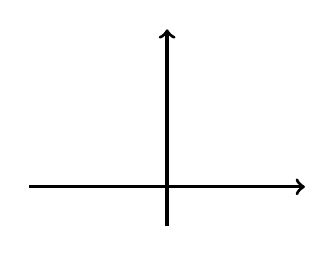
\begin{tikzpicture}[scale=0.5]
\draw[very thick,->] (-3.5,0) -- (3.5,0);
\draw[very thick,->] (0,-1) -- (0,4);
\draw[very thick,color=blue] plot[domain=-1.555:1.555,samples=400] function {(x**2-1)**4};
\end{tikzpicture}

\item $F(x) = x^2(8-x^2)$ 

\begin{tikzpicture}[scale=0.5]
\draw[very thick,->] (-4,0) -- (4,0);
\draw[very thick,->] (0,-3) -- (0,3);
\draw[very thick,color=blue] plot[domain=-3.1:3.1,samples=400] function {(x**2*(8-x**2))/10};
\end{tikzpicture}
\setcounter{enumCount}{\theenumi}
\end{enumerate}
\end{multicols}

\vfill

\begin{enumerate}
\setcounter{enumi}{\theenumCount}
\item A ball thrown in the air has a height of $h(t) = 6 + 32 t - 16t^2$ feet, where $t$ is time in seconds.  How high is the ball at the highest point in its trajectory?
\vfill
\vfill
\vfill
\setcounter{enumCount}{\theenumi}
\end{enumerate}

\newpage
\noindent
\textit{Make a table of $x$ and $y$ values at the critical points and endpoints for each of the following functions.  Indicate which points are the absolute max \& min of each function.}

\begin{enumerate}
\setcounter{enumi}{\theenumCount}
\item $\ds y= \frac{1}{3}x^{3}-9x+2$ on $[0,4]$.
\vfill


\item $\ds y = x + \frac{9}{x}$ on $[1,10]$.
\vfill




\item $\ds f(x) = x^2(3-x)$ on $[0,4]$.
\vfill




%\item The average cost of running a factory is $AC(x) = \dfrac{600}{x} - 5 + \dfrac{x}{6}$, where $x$ is the level of production. This function has one critical point at $x =60$.  Use the second derivative test to show that $x = 60$ minimizes the average cost.   
%\vfill

\noindent
\item A potato farmer estimates that they can get \$8 per bushel for their potatoes on July 1st.  On July 1st, the farmer has 60 bushels of potatoes in the field.  For each day the farmer waits to harvest, the price of potatoes will fall by 10 cents per bushel.  But if the farmer waits, they can increase their harvest by 1 bushel of potatoes per day.  Find a formula for the farmer's revenue as a function of the number of days $x$ they wait to harvest.  Hint: \textit{both price and quantity are linear functions of $x$.  }
\vfill


\item Continuing the last problem, how many days should the farmer wait to harvest their potatoes if they want to maximize revenue?  Be sure to justify your answer using either the first or second derivative test. 
\vfill
\vfill


%\item According to postal regulations, the length plus the circumference of a cylindrical package sent by 4th class mail cannot exceed 9 feet.  Let $x$ be the length, and let $r$ be the radius of the package.  So the largest possible cylindrical packages must satisfy this constraint equation: 
%$ x + 2\pi r = 9.$  
%Use this constraint to find a formula for the volume of a cylindrical package as function of radius only.  (Recall that volume of a cylinder is $V=\pi r^2 x$).  
%\begin{flushright}
%\begin{tikzpicture}
%\node (a) [cylinder, shape border rotate=0, draw, minimum height=15mm, minimum width=7.5mm] {};
%\draw [<->] ([yshift=-5pt]a.before bottom) -- ([yshift=-5pt]a.after top) node [midway, below] {$x$};
%\draw [<->] ([xshift=-5pt]a.bottom) -- ([xshift=-8.3pt] a.before bottom) node [midway, left] {$r$};
%\end{tikzpicture}
%\end{flushright}
%
%\item Find the radius that maximizes the volume in the previous problem. 
%\vfill
%
%\item Find the intervals of increase and decrease for the volume function from the previous problem.  \vfill



\setcounter{enumCount}{\theenumi}
\end{enumerate}


\end{document}
